%-----------------------------------------------------------------------
% Beginning of chapter.tex
%-----------------------------------------------------------------------
%
%  This is a sample file for use with AMS-LaTeX.  It provides an example
%  of how to set up a file for a book to be typeset with AMS-LaTeX.
%
%  This is the driver file.  Separate chapters should be included at
%  the end of this file.
%
%  ***** DO NOT USE THIS FILE AS A STARTER FOR YOUR BOOK. *****
%  Follow the guidelines in the file chapter.template.
%
%%%%%%%%%%%%%%%%%%%%%%%%%%%%%%%%%%%%%%%%%%%%%%%%%%%%%%%%%%%%%%%%%%%%%%%%

\documentclass[11pt,a4paper]{memoir}
\chapterstyle{demo}
\epigraphfontsize{\small\itshape}
\setlength\epigraphwidth{8cm}
\setlength\epigraphrule{0pt}
\epigraphfontsize{\small\itshape}
%\includeonly{preface,chap1,biblio}

%\numberwithin{section}{chapter}
%\numberwithin{equation}{chapter}

% Include macros here
%=================================================
% Packages
%=================================================

%\usepackage{fixltx2e}
\usepackage[usenames,dvipsnames]{xcolor}
%\usepackage{fancyhdr}
\usepackage{amsmath,amsfonts,amsbsy,amsgen,amscd,mathrsfs,amssymb,amscd}
\usepackage{amsthm}
\usepackage{bm}
\usepackage{url}
\usepackage[UKenglish]{babel}
\usepackage{eurosym}
\usepackage{tikz}
\usepackage{caption}
\usetikzlibrary{matrix,arrows,shapes,calc,3d}
\usepackage{tikz-3dplot}
\tdplotsetmaincoords{60}{110}
\pgfmathsetmacro{\rvec}{.8}
\pgfmathsetmacro{\thetavec}{30}
\pgfmathsetmacro{\phivec}{60}

\tikzset{mynode/.style = {
    % The shape
    circle,
    % The size
    minimum size=2pt,
    % The color
    draw=black, fill=black}
}
\tikzset{vertex/.style={shape=circle, % style for a vertex
                        minimum size=3pt,
                        fill=gray,
                        inner sep = 0pt}}  

% \usepackage{3dplot}
% \tdplotsetmaincoords{60}{110}
%\usepackage{subfig}
\usepackage{microtype}
\usepackage{enumitem}
\usepackage{listings}
\definecolor{darkblue}{rgb}{0,0,.75}

\usepackage[many]{tcolorbox}
\tcbuselibrary{listings}

\definecolor{light-gray}{rgb}{0.96,0.96,0.96}
\definecolor{kwgreen}{rgb}{0,0.5,0}
\definecolor{cogreen}{rgb}{0.25,0.5,0.5}
\definecolor{mygreen}{rgb}{0,0.5,0.125}
\definecolor{equalsign}{rgb}{0.66,0.13,1}
\definecolor{darkred}{rgb}{0.75,0.16,0.37}

\lstloadlanguages{Python} %use listings with Python
%\lstset{literate={==}{{\color{equalsign}==}} {\*}{{\color{equalsign}\*}}}
%\lstnewenvironment{PseudoCode}[1][]
% the space reserved between for the ``In'' numbers and the code
\newlength\inwd
\setlength\inwd{1.7cm}

\newcounter{ipythcntr}

\newtcblisting{ipythonnb}[1][\theipythcntr]{
  enlarge left by=\inwd,
  width=\linewidth-\inwd,
  enhanced,
  boxrule=0.4pt,
  boxsep=0pt,
  left=2pt,
  top=0pt,
  colback=light-gray,
  listing only,
  top=0pt,
  bottom=0pt,
  arc=1pt,
  overlay={
    \node[
      anchor=north east,
      text width=\inwd,
      font=\footnotesize\ttfamily\color{blue!50!black},
      inner ysep=2.5mm,
      inner xsep=0pt,
      outer sep=0pt
      ] 
      at (frame.north west)
      {\stepcounter{ipythcntr}In [#1]:};
  }
  listing style=Python,
  listing options={
    basicstyle=\scriptsize\ttfamily\color{black},
    language=Python,
    escapechar=£,
    showstringspaces=false,
    commentstyle=\color{cogreen},
    keywordstyle=\bfseries\color{kwgreen},
    stringstyle=\color{darkred},
    numberstyle=\color{kwgreen},
    identifierstyle=\color{black},
    %emph={from,import,as},          % Custom highlighting
    otherkeywords={0,1,2,3,4,5,6,7,8,9,\*,==,<=,>=,+,-,\%},
    emph={*,==,<=,>=,+,-,\%},    
    emphstyle=\color{equalsign},
    extendedchars=true,
  },
}

\newtcblisting{ipythonnbout}[1][\theipythcntr]{
  enlarge left by=\inwd,
  width=\linewidth-\inwd,
  enhanced,
  boxrule=0pt,
  boxsep=0pt,
  left=2pt,
  top=0pt,
  colback=white,
  listing only,
  top=0pt,
  bottom=0pt,
  frame hidden,
  overlay={
    \node[
      anchor=north east,
      text width=\inwd,
      font=\footnotesize\ttfamily\color{red},
      inner ysep=2.5mm,
      inner xsep=0pt,
      outer sep=0pt
      ] 
      at (frame.north west)
      {\stepcounter{ipythcntr}Out [#1]:};
  }
  listing style=Python,
  listing options={
    basicstyle=\scriptsize\ttfamily\color{black},
    language=Python,
    escapechar=£,
    showstringspaces=false,
    commentstyle=\color{cogreen},
    keywordstyle=\bfseries\color{kwgreen},
    stringstyle=\color{darkred},
    numberstyle=\color{kwgreen},
    identifierstyle=\color{black},
    %emph={from,import,as},          % Custom highlighting
%    otherkeywords={as,0,1,2,3,4,5,6,7,8,9,\*,==,<=,>=,+,-},
%    emph={*,==,<=,>=,+,-},    
%    emphstyle=\color{equalsign},
    extendedchars=true,
    %literate={#}{{\#}},
  },
}

\newtcblisting{ipythonnboutno}{
  enlarge left by=\inwd,
  width=\linewidth-\inwd,
  enhanced,
  boxrule=0pt,
  boxsep=0pt,
  left=2pt,
  top=0pt,
  colback=white,
  listing only,
  top=0pt,
  bottom=0pt,
  frame hidden,
  overlay={
    \node[
      anchor=north east,
      text width=\inwd,
      font=\footnotesize\ttfamily\color{red},
      inner ysep=2.5mm,
      inner xsep=0pt,
      outer sep=0pt
      ] 
      at (frame.north west)
      {};
  }
  listing style=Python,
  listing options={
    basicstyle=\scriptsize\ttfamily\color{black},
    language=Python,
    escapechar=£,
    showstringspaces=false,
    commentstyle=\color{cogreen},
    %keywordstyle=\bfseries\color{kwgreen},
    stringstyle=\color{darkred},
    numberstyle=\color{kwgreen},
    identifierstyle=\color{black},
    %emph={from,import,as},          % Custom highlighting
    %otherkeywords={as,0,1,2,3,4,5,6,7,8,9,\[,\]},
    %emph={[,]},    
    %emphstyle=\color{black},
    extendedchars=true,
    %literate={#}{{\#}},
  },
}


%{\lstset{language=Matlab,basicstyle=\small, keywordstyle=\color{darkblue},numbers=none,xleftmargin=.04\textwidth,mathescape,frame=single,#1}}
%{}
%\usepackage[]{algorithm2e}
%\usepackage{mcode}
\usepackage{multicol}

%\usepackage[draft]{changes}
%\definechangesauthor[color=blue]{ml}
%\definechangesauthor[color=red]{da}
% \usepackage{trackchanges}
% \addeditor{ml}
% \addeditor{da}

\definecolor{dark-gray}{gray}{0.3}
\definecolor{dkgray}{rgb}{.4,.4,.4}
\definecolor{dkblue}{rgb}{0,0,.5}
\definecolor{medblue}{rgb}{0,0,.75}
\definecolor{rust}{rgb}{0.5,0.1,0.1}

\usepackage[colorlinks=true]{hyperref}
\hypersetup{urlcolor=Blue}
\hypersetup{citecolor=Black}
\hypersetup{linkcolor=dark-gray}

%\usepackage{setspace}
\usepackage{graphicx}
%\usepackage{multicol}
\usepackage{booktabs,longtable,tabu} % Nice tables
\setlength{\tabulinesep}{1pt}
\usepackage{multirow} % More control over tables
\usepackage{float}
\usepackage[T1]{fontenc}
%\usepackage{quotchap}

% Fonts
\usepackage{times}
%\usepackage{fourier}
%\usepackage[no-math]{fontspec}
%\setmainfont{optima}
%\usepackage{charter}
\usepackage{bm} % boldmath must be called after the package

%=================================================
% Paths
%=================================================

\graphicspath{{figures/}}

%=================================================
% Formatting
%=================================================

%\sloppy % Helps with margin justification

%%% Further font changes
\newcommand{\lang}{\textit}
\newcommand{\titl}{\textsl}
\newcommand{\term}{\emph}

%%% Equation numbering
\numberwithin{equation}{section} 

%%% Typesetting
\providecommand{\mathbold}[1]{\bm{#1}}  % Must be after 'fourier'
                                % package loads
%%% Annotations
\newcommand{\notate}[1]{\textcolor{red}{\textbf{[#1]}}}

%=================================================
% Theorem environment
%=================================================

\newtheorem{bigthm}{Theorem}
\renewcommand{\thebigthm}{\Roman{bigthm}}

\newtheorem{theorem}{Theorem}[section]
\newtheorem{lemma}[theorem]{Lemma}
\newtheorem{sublemma}[theorem]{Sublemma}
\newtheorem{proposition}[theorem]{Proposition}
\newtheorem{fact}[theorem]{Fact}
\newtheorem{result}[theorem]{Result}
\newtheorem{conjecture}[theorem]{Conjecture}
\newtheorem{corollary}[theorem]{Corollary}

\newtheorem{problem}[theorem]{Problem}
\newtheorem{solution}[theorem]{Solution}

\theoremstyle{definition}

\newtheorem{definition}[theorem]{Definition}
\newtheorem{example}[theorem]{Example}
\newtheorem{remark}[theorem]{Remark}

\newenvironment{mainthm}{\par\textsc{Main theorem.}\it}{\par}
\renewcommand{\thebigthm}{\Alph{bigthm}}

%=================================================
% Symbols
%=================================================

%%% Old symbols with new names
\newcommand{\oldphi}{\phi}
\renewcommand{\phi}{\varphi}

\newcommand{\eps}{\varepsilon}
\newcommand{\e}{\varepsilon}

%\newcommand{\oldmid}{\mid}
\renewcommand{\mid}{\mathrel{\mathop{:}}} 

%%% New symbols
\newcommand{\defby}{\overset{\mathrm{\scriptscriptstyle{def}}}{=}}
\newcommand{\half}{\tfrac{1}{2}}
\newcommand{\third}{\tfrac{1}{3}}

\newcommand{\sumnl}{\sum\nolimits}

\newcommand{\defeq}{\ensuremath{\mathrel{\mathop{:}}=}} % Definition-equals
\newcommand{\eqdef}{\ensuremath{=\mathrel{\mathop{:}}}} % Equals-definition

%%% Constants
\newcommand{\cnst}[1]{\mathrm{#1}} 
\newcommand{\econst}{\mathrm{e}}
\newcommand{\iunit}{\mathrm{i}}

\newcommand{\onevct}{\mathbf{e}} % All ones vector
\newcommand{\zerovct}{\vct{0}} % Zero vector

\newcommand{\Id}{\mathbf{I}}
\newcommand{\onemtx}{\bm{1}}
\newcommand{\zeromtx}{\bm{0}}

%%% Sets
\newcommand{\coll}[1]{\mathscr{#1}}
\newcommand{\sphere}[1]{S^{#1}}
\newcommand{\ball}[1]{B^{#1}}
\newcommand{\Grass}[2]{\mathbb{G}(#1,#2)}
\providecommand{\mathbbm}{\mathbb} % In case we don't load bbm
\newcommand{\Rplus}{\mathbbm{R}_{+}}
\newcommand{\R}{\mathbbm{R}}
\newcommand{\C}{\mathbbm{C}}
\newcommand{\N}{\mathbbm{N}}
\newcommand{\FF}{\mathbbm{F}}
\newcommand{\struct}{\mathcal{S}}

% Group theory
\newcommand{\stab}{\mathrm{stab}}

% Algebra
\newcommand{\End}{\mathrm{End}}
\newcommand{\Hom}{\mathrm{Hom}}
\newcommand{\Mult}{\mathrm{Mult}}

% Set operations
\newcommand{\polar}{\circ}
\newcommand{\closure}{\overline}
\newcommand{\prtensor}{\,\hat{\otimes}\,}

%%% Real and complex analysis
\newcommand{\abs}[1]{\left\vert {#1} \right\vert}
\newcommand{\abssq}[1]{{\abs{#1}}^2}

\newcommand{\sgn}[1]{\operatorname{sgn}{#1}}
\newcommand{\real}{\operatorname{Re}}
\newcommand{\imag}{\operatorname{Im}}
\newcommand{\pos}{\operatorname{Pos}}
\newcommand{\shrink}{\operatorname{Shrink}}

\newcommand{\diff}[1]{\mathrm{d}{#1}}
\newcommand{\idiff}[1]{\, \diff{#1}}

\newcommand{\gradd}{\mathrm{grad }} % Conflicts w/SIAM styles?
\newcommand{\divv}{\mathrm{div }}
\newcommand{\subdiff}{\partial}

%%% Optimization

\newcommand{\minimize}{\text{minimize}\quad}
\newcommand{\maximize}{\text{maximize}\quad}
\newcommand{\subjto}{\quad\text{subject to}\quad}
\newcommand{\find}{\text{find}\quad}
\newcommand{\suchthat}{\quad\text{such that}\quad}

\newcommand{\argmin}{\operatorname*{arg\; min}}
\newcommand{\argmax}{\operatorname*{arg\; max}}
\newcommand{\dom}{\mathrm{dom} }

%%% Probability & measure

\newcommand{\Prob}{\mathbbm{P}}
\newcommand{\Probe}[1]{\Prob\left({#1}\right)}
\newcommand{\Expect}{\operatorname{\mathbb{E}}}

\newcommand{\St}{\operatorname{St}}

%\newcommand{\normal}{\textsc{Normal}}
\newcommand{\normal}{N}
\newcommand{\uniform}{\textsc{Uniform}}
\newcommand{\erf}{\operatorname{erf}}

\DeclareMathOperator{\rvol}{rvol}
\DeclareMathOperator{\Var}{Var}
\DeclareMathOperator{\Gl}{Gl}
\newcommand{\diag}{\operatorname{diag}}

%%% Vector and matrix operators
\newcommand{\vct}[1]{\mathbold{#1}}
\newcommand{\mtx}[1]{\mathbold{#1}}
\newcommand{\Eye}{\mathbf{I}}

\newcommand{\transp}[1]{#1^{T}}
\newcommand{\trans}{\top}
\newcommand{\adj}{*}
\newcommand{\psinv}{\dagger}

\newcommand{\lspan}[1]{\operatorname{span}{#1}}

\newcommand{\range}{\operatorname{range}}
\newcommand{\colspan}{\operatorname{colspan}}

%\newcommand{\rank}{\operatorname{rank}}
\newcommand{\nullity}{\operatorname{null}}
%\newcommand{\ker}{\operatorname{ker}}
\newcommand{\im}{\operatorname{im}}
%\newcommand{\span}{\operatorname{span}}

%\newcommand{\diag}{\operatorname{diag}}
\newcommand{\trace}{\operatorname{tr}}

\newcommand{\supp}[1]{\operatorname{supp}(#1)}
\newcommand{\sign}[1]{\operatorname{sign}(#1)}

\newcommand{\smax}{\sigma_{\max}}
\newcommand{\smin}{\sigma_{\min}}

\newcommand{\nnz}{\operatorname{nnz}}
\renewcommand{\vec}{\operatorname{vec}}

\newcommand{\Proj}{\ensuremath{\mtx{\Pi}}} % Projection operator

%%% Semidefinite orders
\newcommand{\psdle}{\preccurlyeq}
\newcommand{\psdge}{\succcurlyeq}

\newcommand{\psdlt}{\prec}
\newcommand{\psdgt}{\succ}

%%% Mensuration: inner products and norms

% TeX does not like either \newcommand or \renewcommand for these
% two macros.  There is probably a good reason not to use them via
% \def, but I don't know it.  
%\newcommand{\<}{\langle} 
%\newcommand{\>}{\rangle}
\newcommand{\ip}[2]{\langle {#1}, {#2} \rangle}
% --deleted the \left and \right-- Dennis
% \newcommand{\ip}[2]{\left\langle {#1},\ {#2} \right\rangle}
\newcommand{\absip}[2]{\abs{\ip{#1}{#2}}}
\newcommand{\abssqip}[2]{\abssq{\ip{#1}{#2}}}
\newcommand{\tworealip}[2]{2 \, \real{\ip{#1}{#2}}}

%\newcommand{\norm}[1]{\left\Vert {#1} \right\Vert}
\newcommand{\norm}[1]{\Vert {#1}\Vert}
\newcommand{\normsq}[1]{\norm{#1}^2}

\newcommand{\lone}[1]{\norm{#1}_{\ell_1}}
\newcommand{\smlone}[1]{\|#1\|_{\ell_1}}
\newcommand{\linf}[1]{\norm{#1}_{\ell_\infty}}
\newcommand{\sone}[1]{\norm{#1}_{S_1}}
\newcommand{\snorm}[1]{\sone{#1}}
\newcommand{\wnnorm}[1]{\norm{#1}_{*,\vct{w}}}
\newcommand{\wnnormd}[1]{\norm{#1}^*_{\vct{w}}}
\DeclareMathOperator{\dist}{dist}

% Fixed-size inner products and norms are useful sometimes
\newcommand{\smip}[2]{\bigl\langle {#1}, \ {#2} \bigr\rangle}
\newcommand{\smabsip}[2]{\bigl\vert \smip{#1}{#2} \bigr\vert}
\newcommand{\smnorm}[2]{{\bigl\Vert {#2} \bigr\Vert}_{#1}}

% Specific norms that are used frequently
\newcommand{\enormdangle}{{\ell_2}}
\newcommand{\enorm}[1]{\norm{#1}}
\newcommand{\enormsm}[1]{\enorm{\smash{#1}}}

\newcommand{\enormsq}[1]{\enorm{#1}^2}

\newcommand{\fnorm}[1]{\norm{#1}_{\mathrm{F}}}
\newcommand{\fnormsq}[1]{\fnorm{#1}^2}

\newcommand{\pnorm}[2]{\norm{#2}_{#1}}
%\newcommand{\snorm}[1]{\norm{#1}_*}

\newcommand{\triplenorm}[1]{\left\vert\!\left\vert\!\left\vert {#1} \right\vert\!\right\vert\!\right\vert} 

\newcommand{\flag}[2]{{#1 \brack #2}}

% Special cones
\newcommand{\Feas}{\mathcal{F}}
\newcommand{\Desc}{\mathcal{D}}

\newcommand{\sdim}{\delta}
\newcommand{\sdimw}{\delta^*}
% \newcommand{\sdimw}{\tilde{\delta}}
\newcommand{\ddt}[1]{\dot{#1}}
\DeclareMathOperator{\Circ}{Circ}

%%% Differential geometry
\newcommand{\Cinf}{C^{\infty}}
\newcommand{\Tensf}{\mathcal{T}}
\newcommand{\Vbundle}{\mathcal{X}}
\newcommand{\Christ}[3]{\Gamma_{{#1}{#2}}^{#3}}

% Stuff to be sorted in somewhere
\DeclareMathOperator{\Lip}{Lip}

\newcommand{\IR}{\mathbbm{R}}
\newcommand{\veps}{\varepsilon}
\newcommand{\mA}{\mathcal{A}}
\newcommand{\mB}{\mathcal{B}}
\newcommand{\mC}{\mathcal{C}}
\newcommand{\mD}{\mathcal{D}}
\newcommand{\mE}{\mathcal{E}}
\newcommand{\mI}{\mathcal{I}}
\newcommand{\mM}{\mathcal{M}}
\newcommand{\mN}{\mathcal{N}}
\newcommand{\mL}{\mathcal{L}}
\newcommand{\mV}{\mathcal{V}}
\newcommand{\bface}{\overline{\mathcal{F}}}
\newcommand{\face}{\mathcal{F}}
\newcommand{\relint}{\operatorname{relint}}
\newcommand{\relcl}{\operatorname{relcl}}
\newcommand{\cone}{\operatorname{cone}}
\newcommand{\lin}{\operatorname{lin}}
\newcommand{\Gr}{\operatorname{Gr}}
\newcommand{\powerset}{\mathscr{P}}
\newcommand{\hd}{{\operatorname{hd}}}
\newcommand{\inter}{{\operatorname{int}}}
\newcommand{\conv}{\operatorname{conv}}
\newcommand{\clconv}{\overline{\conv}}
\newcommand{\cl}{\operatorname{cl}}
\newcommand{\bd}{\operatorname{bd}}

\newcommand{\GL}{\operatorname{GL}}

% \newcommand{\tb}{\stackrel{0}{\to}}
\newcommand{\tb}{\,\,\mathring{\to}\,\,}
% \newcommand{\tdash}{\,\,\overset{e}{\to}\,\,}
% \newcommand{\tdash}{\,\,\overset{a}{\to}\,\,}
\newcommand{\tdash}{\overset{a}{\to}}

\newcommand{\K}{\mathcal{K}}
\newcommand{\B}{\mathcal{B}}
\newcommand{\F}{\mathcal{F}}
\newcommand{\D}{\mathcal{D}}
\renewcommand{\P}{\mathcal{P}}
\DeclareMathOperator{\id}{id}
\DeclareMathOperator{\gr}{gr}
\newcommand{\vp}{\varphi}
\newcommand{\maxp}{{\max}_p}
\DeclareMathOperator{\spa}{span}
\DeclareMathOperator{\vol}{vol}
\DeclareMathOperator{\ima}{im}
\DeclareMathOperator{\rk}{rk}

\newcommand{\Ren}{\mathcal{R}}
\newcommand{\T}{\mathcal{T}}
% ADJUST THE FOLLOWING
% \newcommand{\resTMP}[2]{#1,#2}
\newcommand{\resTMP}[2]{#1\to#2}
% 
\newcommand{\res}[3]{\vct{#1}_{\resTMP{#2}{#3}}}
\newcommand{\nres}[3]{\|\vct{#1}\|_{\resTMP{#2}{#3}}}
\newcommand{\sres}[3]{\sigma_{\resTMP{#2}{#3}}(\vct{#1})}
\newcommand{\csres}[3]{\overline{\sigma}_{\resTMP{#2}{#3}}(\vct{#1})}
\newcommand{\kres}[3]{\kappa_{\resTMP{#2}{#3}}(\vct{#1})}
% transpose
\newcommand{\rest}[3]{\vct{#1}^T_{\resTMP{#2}{#3}}}
\newcommand{\nrest}[3]{\|\vct{#1}^T\|_{\resTMP{#2}{#3}}}
\newcommand{\srest}[3]{\sigma_{\resTMP{#2}{#3}}(\vct{#1}^T)}
\newcommand{\csrest}[3]{\overline{\sigma}_{\resTMP{#2}{#3}}(\vct{#1}^T)}
\newcommand{\srestm}[3]{\sigma_{\resTMP{#2}{#3}}(-\vct{#1}^T)}
\newcommand{\krest}[3]{\kappa_{\resTMP{#2}{#3}}(\vct{#1}^T)}
\newcommand{\nresdag}[3]{\|\vct{#1}^\dagger\|_{\resTMP{#2}{#3}}}

\newcommand{\RCD}[3]{\Ren_{#2,#3}(\vct{#1})}
% \newcommand{\RCD}[3]{\Ren_{\resTMP{#2}{#3}}(\vct{#1})}

\newcommand{\DA}{\vct{\Delta A}}

%
\newcommand{\Rmm}{R_{\mathrm{mm}}}

\newcommand{\rbinom}[2]{\genfrac{[}{]}{0pt}{}{#1}{#2}}
\newcommand{\trbinom}[2]{{\textstyle\genfrac{[}{]}{0pt}{}{#1}{#2}}}

\newcommand{\comm}[1]{\textcolor{red}{\textbf{[#1]}}}
\newcommand{\rant}[1]{\textcolor{blue}{\textbf{[#1]}}}
%

\newcommand{\llangle}{\langle\hspace{-1.5pt}\langle}  % this is actually contained in mnsymbol, but loading this package causes trouble...
\newcommand{\rrangle}{\rangle\hspace{-1.5pt}\rangle}  % this is actually contained in mnsymbol, but loading this package causes trouble...

\newcommand{\Res}{\mathrm{Res}}
\newcommand{\Oh}{\mathcal{O}}
\newcommand{\Mbar}{\overline{M}}
\newcommand{\second}{\mathrm{II}}
\newcommand{\nablabar}{\overline{\nabla}}
\newcommand{\expm}{\mathrm{exp}}
\newcommand{\Rc}{\mathrm{Rc}}
\newcommand{\NJ}{\mathrm{NJ}}
% %\newcommand{\GL}[1]{\mathrm{GL}(#1)}

\newcommand{\cover}{\lessdot}

% Semidefinite programming
\newcommand{\Sym}{\mathcal{S}}
\newcommand{\SDP}{\mathcal{S}_+}
\newcommand{\psd}{\succeq}
\newcommand{\bdot}{\bullet}

%\renewcommand{\chaptername}{}
%\renewcommand{\thechapter}{}

\begin{document}
\numberwithin{section}{chapter}
\numberwithin{equation}{chapter}
\numberwithin{theorem}{chapter}

\lstset{language=Matlab}

%\frontmatter
%\title{Convex Optimization}

%    Information for first author
%\author{Martin Lotz}
%    Address of record for the research reported here

%\address{School of Mathematics\\ The University of Manchester\\ Alan Turing Building, Oxford Road\\ Manchester M139PL}

%\email{martin.lotz@manchester.ed.uk}
%\urladdr{http://www.maths.manchester.ac.uk/\textasciitilde mlotz}

%\date{\today}

%\maketitle

%\newpage 

%\tableofcontents

%\include{preface}

\mainmatter

%\include{notation}
%-----------------------------------------------------------------------
% Beginning of chap2.tex
%-----------------------------------------------------------------------
%
%  AMS-LaTeX sample file for a chapter of a monograph, to be used with
%  an AMS monograph document class.  This is a data file input by
%  chapter.tex.
%
%  Use this file as a model for a chapter; DO NOT START BY removing its
%  contents and filling in your own text.
% 
%%%%%%%%%%%%%%%%%%%%%%%%%%%%%%%%%%%%%%%%%%%%%%%%%%%%%%%%%%%%%%%%%%%%%%%%


\chapter*{Lecture 7}
\addcontentsline{toc}{chapter}{Lecture 6}
\addtocounter{chapter}{7}
\addtocounter{section}{0}
%\numberwithin{section}{chapter}
\numberwithin{equation}{chapter}
\numberwithin{theorem}{chapter}

% \epigraph{}{--- \textup{}}
\epigraph{``[A]lmost every ``convex'' idea can be explained by a two-dimensional picture.''}{--- \textup{Alexander Barvinok}}

In this lecture we begin our study of the theory underlying constrained convex optimization. One way to define a {\em convex optimization problem} is
\begin{align*}
\begin{split}
 \minimize & f(\vct{x})\\
 \subjto & f_1(\vct{x})\leq 0\\
 & \cdots \\
 & f_m(\vct{x})\leq 0\\
 & \vct{x}\in \Omega
 \end{split}
\end{align*}
where $f,f_1,\dots,f_m\colon \R^n\to \R$ are {\em convex} functions and $\Omega\subseteq \R^n$ is a {\em convex} set. The special case where the $f$ and the $f_i$ are linear functions and $\Omega=\R^n$ is known as linear programming, and is studied first. Before embarking on the study of models and algorithms for convex optimization, we need to study convex sets in more depth.

\section{Convex sets}
We recall the definition of a convex set.
\begin{definition}
 A set $C\subseteq \R^n$ is a {\em convex set}, if for all $\vct{x},\vct{y}\in C$ and $\lambda\in [0,1]$, $\lambda\vct{x}+(1-\lambda)\vct{y}\in C$. In words, for every two points in $C$, the line joining them is also in $C$. A compact (closed and bounded) convex set is called a {\em convex body}.
\end{definition}

\begin{figure}[h!]
\centering
\begin{tikzpicture}[thick,rotate=15,scale=0.8]
\filldraw[color=black, fill=blue!5, very thick, rotate=15](0,0) ellipse (2 and 1.2);

\node (A1) at (-1,0)  [label=180:$\vct{x}$] {};
\node (A2) at (1,0)   [label=0:$\vct{y}$] {};
\filldraw[black] (-0.9,0) circle (2pt);
\filldraw[black] (0.9,0) circle (2pt);

\draw[color=blue,thick] (A1) -- (A2);
\end{tikzpicture}
\end{figure}

We will denote by $\mathcal{C}(\R^n)$ the collection of convex sets and by $\mathcal{K}(\R^n)$ the collection of convex bodies. The following Lemma is left as an exercise.

\begin{lemma}
 Let $C,D\in \mathcal{C}(\R^n)$ be convex sets. Then the following are also convex.
 \begin{itemize}
  \item $\displaystyle C\cap D$;
  \item $\displaystyle C+D=\{\vct{x}+\vct{y} \mid \vct{x}\in C, \vct{y}\in D\}$;
  \item $\displaystyle \mtx{A}C=\{\mtx{A}\vct{x} \mid \vct{x}\in C\}$, where $\mtx{A}\in \R^{m\times n}$.
 \end{itemize}
\end{lemma}

The {\em convex hull} $\conv{S}$ of a set $S$ is the intersection of all convex sets containing $S$. Clearly, if $S$ is convex, then $S=\conv{S}$.

\begin{example}
 Let $S=\{(1,1)^{\trans},(1,-1)^{\trans},(-1,1)^{\trans},(-1,-1)^{\trans},(0,0)^{\trans}\}$. The convex hull of this set is the square.
 \begin{figure}[h!]
\centering
\begin{tikzpicture}[thick,scale=1]
\node (A1) at (-1.1,-1.1)  [label=195:{(-1,-1)}] {};
\node (A2) at (1.1,1.1)   [label=45:{(1,1)}] {};
\node (A3) at (-1,1)  [label=135:{(-1,1)}] {};
\node (A4) at (1,-1)   [label=-45:{(1,-1)}] {};
\node (A5) at (0,0)   [label=90:{(0,0)}] {};
\draw[color=black!15, fill=blue!5, thick, rounded corners=2pt, dashed] (A1) rectangle (A2);
\filldraw[black] (1,1) circle (2pt);
\filldraw[black] (1,-1) circle (2pt);
\filldraw[black] (-1,1) circle (2pt);
\filldraw[black] (-1,-1) circle (2pt);
\filldraw[black] (0,0) circle (2pt);
\end{tikzpicture}
\caption{A convex hull of five points.}
\end{figure}
\end{example}

A {\em convex combination} of points $\vct{x}_1,\dots,\vct{x}_k$ is a linear combination
\begin{equation*}
 \sum_{i=1}^k \lambda_i \vct{x}_i
\end{equation*}
such that $\lambda_i\geq 0$ and $\sum_{i=1}^k \lambda_i = 1$. It can be shown inductively that convex sets are closed under convex combinations: any convex combination of points in $C\in \mathcal{C}(\R^n)$ is still in $C$. In fact, the set of all convex combinations of points in a set $S$ is the convex hull of $S$.

\begin{lemma}
 Let $S$ be a set. Then 
 \begin{equation*}
  \conv{S} = \{\vct{x}\in \R^n \mid \vct{x}=\sum_{i=1}^k \lambda_i \vct{x}_k, \ \vct{x}_i\in S, \ \sum_{i=1}^k \lambda_i = 1, \ \lambda_i\geq 0\}.
 \end{equation*}
\end{lemma}

\begin{example}
A hyperplane, defined as the solution set of one linear equations,
\begin{equation*}
 H = \{\vct{x} \mid \ip{\vct{a}}{\vct{x}} = b\},
\end{equation*}
is a convex set.
Define the halfspaces $H_+$ and $H_-$ as the two sides that $H$ divides $\R^n$ into:
\begin{equation*}
 H_- = \{\vct{x}\mid \ip{\vct{a}}{\vct{x}}\leq b\}, \quad H_+ = \{\vct{x}\mid \ip{\vct{a}}{\vct{x}}\geq b\}
\end{equation*}
These are also convex sets. 
\begin{figure}[h!]
\centering
\begin{tikzpicture}[thick,rotate=-45]
\coordinate (A1) at (-1.1,0);
\coordinate (A2) at (1.1,0);
\coordinate (A3) at (0,-1.2);
\coordinate (A4) at (0,1);
\coordinate (A5) at (1.1,-1);

\draw[color=black!0, fill=blue!5, thick, dashed] (A1) rectangle (A5);
\draw[color=black, thick] (A1) -- (A2);
\draw[color=black, thick,->] (A3) -- (A4);
\filldraw[black] (A3) circle (2pt);

\node (A) at (0.2,1) [label=90:$\vct{a}$] {};
\node (H) at (1,0) [label=0:{$\ip{\vct{a}}{\vct{x}}=b$}] {};
\node (Hm) at (-1.2,-0.5) [label=270:{$\ip{\vct{a}}{\vct{x}}\leq b$}] {};
\end{tikzpicture}
\caption{Hyperplane and halfspace}
\end{figure}
\end{example}

\begin{example}
 Euclidean balls and ellipsoids are common examples of convex sets. Let $\mtx{P}$ be a positive semidefinite symmetric matrix. Then an ellipsoid with center $\vct{x}_0$ is a set of the form
 \begin{equation*}
  \mathcal{E} = \{\vct{x} \mid \ip{\vct{x}-\vct{x}_0}{\mtx{P}^{-1}(\vct{x}-\vct{x}_0)}\leq 1\}.
 \end{equation*}
A Euclidean unit ball is the special case $\mtx{P}=\mtx{I}$.
\begin{figure}[h!]
\centering
\begin{tikzpicture}[thick,rotate=15,scale=0.8]
\filldraw[color=black, fill=blue!5, very thick, rotate=15](0,0) ellipse (2 and 1.2);

\node (A1) at (0,0)  [label=45:{$\vct{x}_0$}] {};
\filldraw[black] (0,0) circle (2pt);
\end{tikzpicture}
\caption{An ellipse}
\end{figure}
\end{example}

\begin{example}
 A {\em convex cone} is a set $C$ such that for all $\vct{x},\vct{y}$ and $\lambda\geq 0, \mu\geq 0$,
 $\lambda \vct{x}+\mu \vct{y}\in C$. It is easily verified that such a set is convex. Three important cones are the following:
 \begin{enumerate}
  \item The non-negative orthant $\R^d_{+}=\{\vct{x}\in \R^d \mid x_i\geq 0, 1\leq i\leq d\}$,
  \item The second order (ice cream) cone (or Lorentz cone)
  \begin{equation*}
   C_{\alpha} = \{\vct{x} \mid \sum_{i=1}^{d-1}x_i^2\leq x_d^2\},
  \end{equation*}
  \item The cone $\mathcal{S}_{+}^d$ of positive semidefinite symmetric matrices.
 \end{enumerate}
\begin{figure}[h!]
\centering
 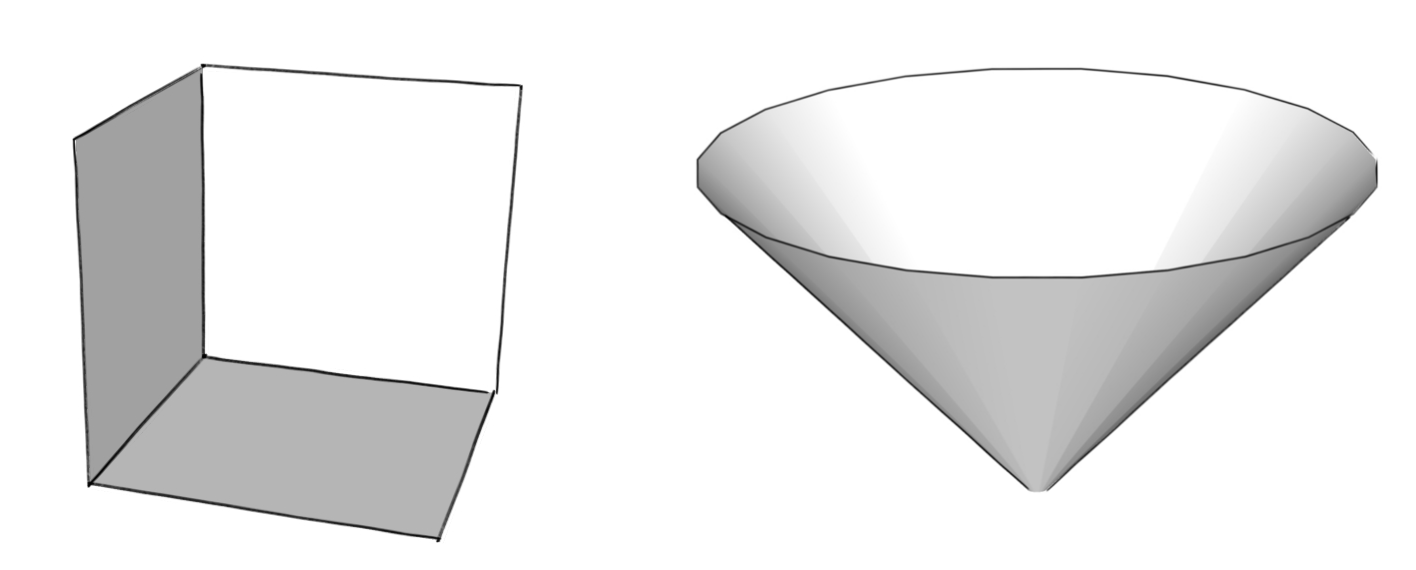
\includegraphics[width=0.6\textwidth]{images/cones.png}
 \caption{The orthant and the second order cone}
\end{figure}

\end{example}


Possibly the most important result in convex geometry is the {\em hyperplane separation theorem}.  We first need the following.

\begin{lemma}\label{le:obtuse}
 Let $C$ be a non-empty convex set and $\vct{x}\not\in C$. Then there exists a point $\vct{y}\in C$ that minimizes the distance $\norm{\vct{x}-\vct{y}}$. Moreover, for all $\vct{z}\in C$ we have
 \begin{equation*}
  \ip{\vct{z}-\vct{y}}{\vct{x}-\vct{y}}\leq 0.
 \end{equation*}
In words, the vectors $\vct{z}-\vct{y}$ and $\vct{x}-\vct{y}$ form an obtuse angle.
\end{lemma}

\begin{figure}[h!]
\centering
\begin{tikzpicture}[thick,rotate=30,scale=0.8]
\filldraw[color=black, fill=blue!5, very thick](0,0) ellipse (2 and 1.2);
\node (A1) at (0,-3)  [label=0:{$\vct{x}$}] {};
\node (A2) at (0,-1.2)  [label=90:{$\vct{y}$}] {};
%\node (A3) at (0,-2.5)  [label=180:{$\vct{a}$}] {};
\node (A4) at (-1,0)  [label=180:{$\vct{z}$}] {};
\filldraw[black] (0,-3) circle (2pt);
\filldraw[black] (0,-1.2) circle (2pt);
\filldraw[black] (-1,0) circle (2pt);
\draw[color=black, thick, <-] (0,-2.9) -- (0,-1.2);
\draw[color=black, thick, <-] (-0.9,-0.1) -- (0,-1.2);
\end{tikzpicture}
\caption{Internal and external directions} \label{fig:neg}
\end{figure}

\begin{proof}
 Since $C\neq \emptyset$, there exists $r>0$ such that the ball $B(\vct{x},r):=\{\vct{y}\in \R^d \mid \norm{\vct{y}-\vct{x}}\leq \e\}$ intersected with $C$ is not empty. Since $K:=C\cap B(\vct{x},r)$ is compact (closed and bounded) and the function $\norm{\vct{y}-\vct{x}}$ is continuous on $K$, it has a minimizer $\vct{y}\in K$. For the second claim, note that since $C$ is convex, for every $\lambda\in [0,1]$,
 \begin{equation*}
  \vct{w} = \lambda \vct{z}+(1-\lambda)\vct{y} \in C.
 \end{equation*}
For the distance between $\vct{z}$ and $\vct{x}$ we then get
\begin{align*}
 \norm{\vct{w}-\vct{x}}^2  &= \norm{\lambda\vct{z}+(1-\lambda) \vct{y}-\vct{x}}^2 = \norm{\lambda (\vct{z}-\vct{y})-(\vct{x}-\vct{y})}^2\\
 &= \lambda^2\norm{\vct{z}-\vct{y}}^2-2\lambda \ip{\vct{z}-\vct{y}}{\vct{x}-\vct{y}}+\norm{\vct{x}-\vct{y}}^2.
\end{align*}
We now prove the claim by contradition. Assume $\ip{\vct{z}-\vct{y}}{\vct{x}-\vct{y}}>0$. Then we can choose $\lambda$ such that
\begin{equation*}
 0< \lambda < \min\left\{ \frac{2\ip{\vct{x}-\vct{y}}{\vct{z}-\vct{y}}}{\norm{\vct{z}-\vct{y}}^2} , 1\right\}.
\end{equation*}
With such a $\lambda$ we get
\begin{equation*}
 \norm{\vct{w}-\vct{x}}^2 = \lambda^2\norm{\vct{z}-\vct{y}}^2-2\lambda \ip{\vct{z}-\vct{y}}{\vct{x}-\vct{y}}+\norm{\vct{x}-\vct{y}}^2 < \norm{\vct{x}-\vct{y}}^2.
\end{equation*}
This inequality, however, contradicts the assumption that $\vct{y}$ is a closest point, so that
$\ip{\vct{z}-\vct{y}}{\vct{x}-\vct{y}}\leq 0$ has to hold.
\end{proof}

In what follows write $\inter S$ for the {\em interior} of a set $S$.

\begin{theorem}
 Let $C$ be a closed convex set and $\vct{x}\not\in C$. Then there exists a hyperplane $H$ such that $C\subset \inter H_-$ and $\vct{x}\in \inter H_+$. 
\end{theorem}

\begin{figure}[h!]
\centering
\begin{tikzpicture}[thick,rotate=30,scale=0.8]
\filldraw[color=black, fill=blue!5, very thick](0,0) ellipse (2 and 1.2);

\node (A1) at (0,-2)  [label=0:{$\vct{x}$}] {};
\filldraw[black] (0,-2) circle (2pt);
\draw[color=black, thick] (-3,-1.5) -- (3,-1.5);
\end{tikzpicture}
\caption{A separating hyperplane}
\end{figure}

\begin{proof}
 Let $\vct{y}\in C$ be a nearest point to $\vct{x}$ in $C$, i.e., a point such that for all other $\vct{z}\in C$, $\norm{\vct{x}-\vct{y}}\leq \norm{\vct{x}-\vct{z}}$. Define
 \begin{equation*}
  \vct{a}= \vct{x}-\vct{y}, \quad b = (\norm{\vct{x}}^2-\norm{\vct{y}}^2)/2.
 \end{equation*}
We aim to show that $\ip{\vct{a}}{\vct{x}} = b$ defines a separating hyperplane. 

For this we have to show that
\begin{enumerate}
 \item $\ip{\vct{a}}{\vct{x}}>b$;
 \item For all $\vct{z}\in C$, $\ip{\vct{a}}{\vct{z}}<b$.
\end{enumerate}
For (1), note that 
\begin{equation*}
 \ip{\vct{a}}{\vct{x}} = \ip{\vct{x}-\vct{y}}{\vct{x}}>\ip{\vct{x}-\vct{y}}{\vct{x}}-\frac{1}{2}\norm{\vct{x}-\vct{y}}^2 = \frac{1}{2}(\norm{\vct{x}}^2-\norm{\vct{y}}^2) = b.
\end{equation*}
To prove (2), assume on the contrary that there exists a $\vct{z}\in C$ such that $\ip{\vct{a}}{\vct{z}}\geq b$. We know that the point $\vct{y}\in C$ satisfies the inequality (2), since
\begin{equation*}
 \ip{\vct{a}}{\vct{y}} < \ip{\vct{a}}{\vct{y}}+\frac{1}{2}\norm{\vct{a}}^2 = \ip{\vct{a}}{\vct{y}}+\frac{1}{2}\norm{\vct{x}-\vct{y}}^2 = b.
\end{equation*}
Therefore, 
\begin{equation*}
 \ip{\vct{a}}{\vct{z}-\vct{y}} = \ip{\vct{a}}{\vct{z}}-\ip{\vct{a}}{\vct{y}} > b-b = 0,
\end{equation*}
but this contradict Lemma~\ref{le:obtuse}. We therefore conclude $\ip{\vct{a}}{\vct{z}}<b$. The separating hyperplane $H$ is thus defined by the equation $\ip{\vct{a}}{\vct{x}}=b$. 
\end{proof}

% %-----------------------------------------------------------------------
% % End of chap1.tex
% %-----------------------------------------------------------------------


%\appendix
%\include{appendix1}

%\backmatter
%\include{biblio}
%\include{index}
\end{document}

%-----------------------------------------------------------------------
% End of chapter.tex
%-----------------------------------------------------------------------
